
                \documentclass[a4paper,11pt,fleqn]{article}
                \usepackage[utf8]{inputenc}
                \usepackage[left=1cm,right=0.5cm,top=0.5cm,bottom=2cm]{geometry}

                \usepackage{bfcours}
                \usepackage{datatool}
                \usepackage{geometry}
                \usepackage{pgfplots}
                \pgfplotsset{compat=1.18}
                \usepgfplotslibrary{polar}
                \usepackage{pgfplotstable}
                \usepackage{float}
                \usepackage{multicol}
                \usepackage[most]{tcolorbox}
                \usepackage{hyperref}

                \DTLsetseparator{;} % Assurez-vous que cela correspond au séparateur de votre fichier CSV.
                \hypersetup{
                    pdfauthor={R.Deschamps},
                    pdfsubject={},
                    pdfkeywords={},
                    pdfproducer={LuaLaTeX},
                    pdfcreator={Boum Factory}
                }
                
% Définition d'une nouvelle tcolorbox minimaliste
                \usepackage{siunitx}
                \sisetup{output-decimal-marker={,}} 
                \newcommand\boitesignature[2]{
                \begin{multicols}{2}
                    \begin{tcolorbox}[nobeforeafter,colframe=white, % Couleur de la bordure
                    colback=white, % Couleur de fond
                    boxsep=0pt, % Pas d'espace entre le texte et les bords de la boîte
                    top=0pt, bottom=0pt, left=0pt, right=0pt, % Pas de marges intérieures
                    boxrule=0pt, % Pas de bordure visible
                    height=3cm,
                    arc=0pt, % Coins non arrondis
                    ]
                        #1
                    \end{tcolorbox}
                    
                    \columnbreak
                    
                    \begin{tcolorbox}[nobeforeafter,height=3cm,title=\bfseries Résultat obtenu au contrôle :,halign title=flush left,fonttitle=\bfseries,colbacktitle=black,coltitle=white,colback=white]%red!50!black
                        #2
                    \end{tcolorbox}
                \end{multicols}
                }

                \def\rdifficulty{1}
                \def\points{1}
                \setrdexo{%left skip=1cm,
                display exotitle,
                exo header = tcolorbox,
                %display tags,
                skin = bouyachakka,
                lower ={box=crep},
                display score,
                display level,
                save lower,
                score=\points,
                level=\rdifficulty,
                overlay={\node[inner sep=0pt,
                anchor=west,rotate=90, yshift=0.3cm]%,xshift=-3em], yshift=0.45cm
                at (frame.south west) {\thetags[0]} ;}
                ]%obligatoire
                }
                \setrdcrep{seyes, correction=true, correction color=monrose, correction font = \large\bfseries}
                \title{Analyse du devoir : }
                \author{R.Deschamps}
                \begin{document}
                \setcounter{pagecounter}{0}
                \setcounter{ExoMA}{0}
                \setcounter{prof}{0}
                \chapitre[Prof]{
                analyse%
                }{
                Collège% type_etablissement : Collège,Lycée
                }{
                % nom_etablissement : Amadis Jamyn,Eugène Belgrand
                }{
                %
                }{
                Analyse du devoir : 
                }

                \tableofcontents
                
                \newpage

                
\section{Analyse du devoir du 04/05/2024}

    \subsection{\'Etude de la répartition des résultats}

    %%% debut - Répartition des résultats %%%

    \begin{center}
        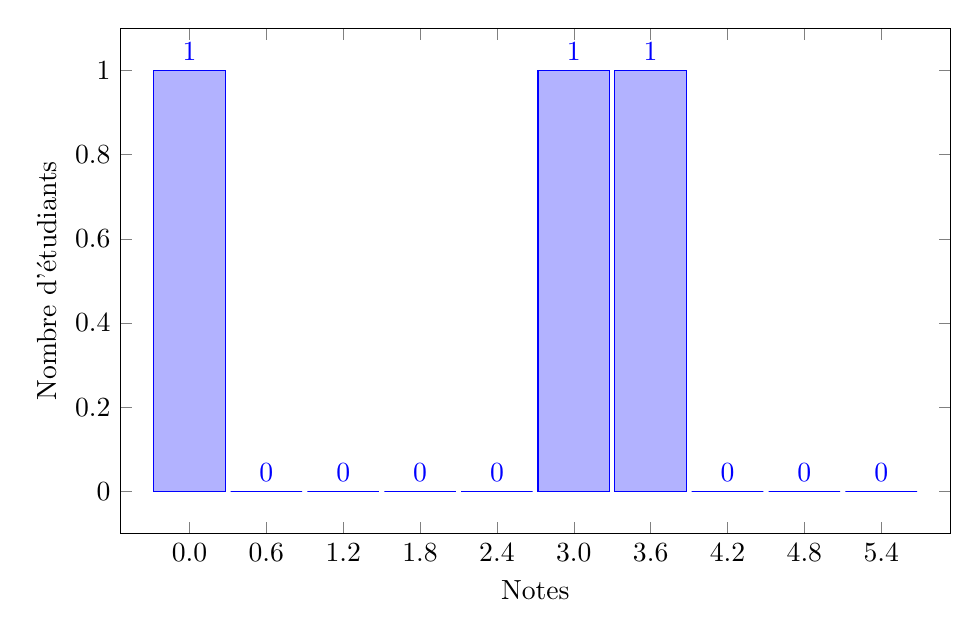
\begin{tikzpicture}
\begin{axis}[
width=\textwidth,
ybar=1.0,
bar width=0.9090909090909092cm,
height=8cm,
ylabel={Nombre d'étudiants},
xlabel={Notes},
xtick=data,
xtick align=inside,
xticklabel style={align=center},
xtick={0.3, 0.9, 1.5, 2.1, 2.7, 3.3, 3.9, 4.5, 5.1, 5.7},
xticklabels={0.0, 0.6, 1.2, 1.8, 2.4, 3.0, 3.6, 4.2, 4.8, 5.4, 6.0},
nodes near coords,
area style,
]
\addplot coordinates {
(0.30, 1) (0.90, 0) (1.50, 0) (2.10, 0) (2.70, 0) (3.30, 1) (3.90, 1) (4.50, 0) (5.10, 0) (5.70, 0) };
\end{axis}
\end{tikzpicture}
    \end{center}

    %%% fin - Répartition des résultats %%%
    
    \subsection{Compétences du devoir}

    %%% debut - tableau %%%
    
    \begin{center}
        \\
\\

    \end{center}

    %%% fin - tableau %%%

\newpage

\subsection{Tableau d'analyse des résultats}

    %%% debut - Tableau des résultats %%%

    
    \begin{center}
        \begin{tcbtab}{c|c|c|c|c|c|c|}
        \hline
        \rowcolor{blue!75!black}\bfseries \color{white}Nom & \bfseries \color{white}Prenom & \bfseries \color{white}Total & \bfseries \color{white}E1  & \bfseries \color{white}E2  & \bfseries \color{white}E3  \\
        \hline

      \rowcolor{blue!10!white}\bfseries ageugeu & \bfseries beubeubeu & \cellcolor{red!15!white} \color{black}\bfseries\num{0} & \num{0}& \num{0}& \num{0} \\
      \hline

      \rowcolor{blue!5!white}\bfseries joeystar & \bfseries Jonathan & \cellcolor{blue!15!white} \color{black}\bfseries\num{3} & \num{0}& \num{3}& \num{0} \\
      \hline

      \rowcolor{blue!10!white}\bfseries littlewood & \bfseries boumbazar & \cellcolor{blue!15!white} \color{black}\bfseries\num{4} & \num{2}& \num{0}& \num{2} \\
      \hline

\end{tcbtab}
\end{center}


    %%% fin - Tableau des résultats %%%

\newpage
    
\subsection{Analyse par exercices}

\begin{multicols}{2}

    %%% debut - explications %%%
    \boite{Commentaires :}{
    
        %%% debut - analyse %%%

        \begin{itemize}
\item Exercices peu réussis : 2, 3
\item Exercices bien réussis : 1
\end{itemize}


        %%% fin - analyse %%%

        
        Note moyenne obtenue au contrôle : \begin{center} $\mathbf{2{,}5/6}$\end{center}
        Explications pour les exercices : 
        \begin{itemize}
            %\item Exercice 1 :\\ 
%\item Exercice 2 :\\ 
%\item Exercice 3 :\\ 
        \end{itemize}
        

    }
    %%% fin - explications %%%
    
    \columnbreak

    %%% debut - tableau %%%
    
    \begin{center}
        \begin{tcbtab}[Statistiques]{c|c|c|c|c}
\hline
 & q1 & Moyenne & q3 & Barème \\ \hline
Exercice 1 & {\scriptsize 0{,}00} & $\mathbf{0{,}67}$ & {\scriptsize 1{,}00} & 1 \\ \hline
Exercice 2 & {\scriptsize 0{,}00} & $\mathbf{1{,}00}$ & {\scriptsize 1{,}50} & 3 \\ \hline
Exercice 3 & {\scriptsize 0{,}00} & $\mathbf{0{,}67}$ & {\scriptsize 1{,}00} & 2 \\ \hline
\end{tcbtab}
    \end{center}

    %%% fin - tableau %%%

    %%% debut - radar %%%
    
    
\begin{center}
    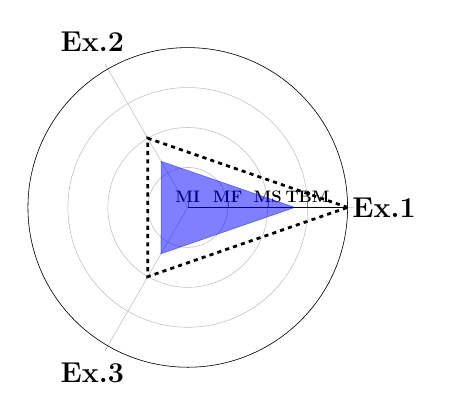
\begin{tikzpicture}[scale=0.5]
        \begin{polaraxis}[
            width=0.8\textwidth,
            xtick={0.0,120.0,240.0},
            xticklabels={\huge \bfseries Ex.1,\huge \bfseries Ex.2,\huge \bfseries Ex.3},
            ymin=0, ymax=100,
            ytick={0,25,50,75,100},
            yticklabels={\large \bfseries MI,\large \bfseries MF,\large \bfseries MS,\large \bfseries TBM, }
        ]
        \addplot+[mark=none,fill=blue,opacity=0.5] coordinates {
            (0.0,67.0)  (120.0,33.333333333333336)  (240.0,33.5)  
        } -- cycle;
        
        \addplot+[mark=none,fill=none,opacity=1,line width = 2pt,dashed,color=black] coordinates {
                    (0.0,0.0)  (120.0,0.0)  (240.0,0.0)  
                } -- cycle;
        
        \addplot+[mark=none,fill=none,opacity=1,line width = 2pt,dashed,color=black] coordinates {
                    (0.0,100.0)  (120.0,50.0)  (240.0,50.0)  
                } -- cycle;
        
        \end{polaraxis}
    \end{tikzpicture}
\end{center}


    %%% fin - radar %%%

\end{multicols}



                \newpage

                
\section{Résultats de AGEUGEU Beubeubeu}

    %%% debut - tableau %%%
    \boitesignature{
    \textbf{Titre : }{''}
    \textbf{Contrôle effectué le : 04/05/2024} \\
    \textbf{Thèmes abordés : }
    }{\begin{center}\bfseries\huge{0/6} \end{center}}

    \begin{center}
        
\begin{tcbtab}[Par exercice :]{|c|c|c|c|}
      \hline
       & \bfseries Exercice 1  & \bfseries Exercice 2  & \bfseries Exercice 3  \\
      \hline
      \bfseries Points  & 0 & 0 & 0 \\
      \hline
      \bfseries Barème  & 1 & 3 & 2 \\
      \hline
\end{tcbtab}

    \end{center}

    %%% fin - tableau %%%

\begin{multicols}{2}

    %%% debut - explications %%%
    \boite{Commentaires :}{
        
            \begin{itemize}

                \item \textbf{Exercice 1} à retravailler.
            \item \textbf{Exercice 2} à retravailler.
            \item \textbf{Exercice 3} à retravailler.
            
            \end{itemize}

    
    }
    %%% fin - explications %%%
    
    \columnbreak

    %%% debut - radar %%%
    
    
\begin{center}
    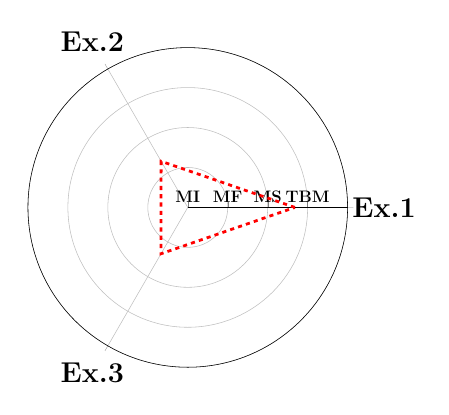
\begin{tikzpicture}[scale=0.5]
        \begin{polaraxis}[
            width=0.8\textwidth,
            xtick={0.0,120.0,240.0},
            xticklabels={\huge \bfseries Ex.1,\huge \bfseries Ex.2,\huge \bfseries Ex.3},
            ymin=0, ymax=100,
            ytick={0,25,50,75,100},
            yticklabels={\large \bfseries MI,\large \bfseries MF,\large \bfseries MS,\large \bfseries TBM, }
        ]
        \addplot+[mark=none,fill=blue,opacity=0.5] coordinates {
            (0.0,0.0)  (120.0,0.0)  (240.0,0.0)  
        } -- cycle;
        
        \addplot+[mark=none,fill=none,opacity=1,line width = 2pt,dashed,color=red] coordinates {
                    (0.0,67.0)  (120.0,33.333333333333336)  (240.0,33.5)  
                } -- cycle;
        
        \end{polaraxis}
    \end{tikzpicture}
\end{center}


    %%% fin - radar %%%

\end{multicols}

                \newpage
                
\section{Résultats de JOEYSTAR Jonathan}

    %%% debut - tableau %%%
    \boitesignature{
    \textbf{Titre : }{''}
    \textbf{Contrôle effectué le : 04/05/2024} \\
    \textbf{Thèmes abordés : }
    }{\begin{center}\bfseries\huge{3/6} \end{center}}

    \begin{center}
        
\begin{tcbtab}[Par exercice :]{|c|c|c|c|}
      \hline
       & \bfseries Exercice 1  & \bfseries Exercice 2  & \bfseries Exercice 3  \\
      \hline
      \bfseries Points  & 0 & 3 & 0 \\
      \hline
      \bfseries Barème  & 1 & 3 & 2 \\
      \hline
\end{tcbtab}

    \end{center}

    %%% fin - tableau %%%

\begin{multicols}{2}

    %%% debut - explications %%%
    \boite{Commentaires :}{
        
            \begin{itemize}

                \item \textbf{Exercice 1} à retravailler.
            \item \textbf{Exercice 3} à retravailler.
            
            \end{itemize}

    
    }
    %%% fin - explications %%%
    
    \columnbreak

    %%% debut - radar %%%
    
    
\begin{center}
    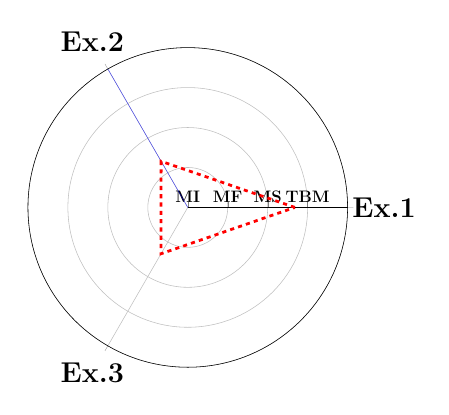
\begin{tikzpicture}[scale=0.5]
        \begin{polaraxis}[
            width=0.8\textwidth,
            xtick={0.0,120.0,240.0},
            xticklabels={\huge \bfseries Ex.1,\huge \bfseries Ex.2,\huge \bfseries Ex.3},
            ymin=0, ymax=100,
            ytick={0,25,50,75,100},
            yticklabels={\large \bfseries MI,\large \bfseries MF,\large \bfseries MS,\large \bfseries TBM, }
        ]
        \addplot+[mark=none,fill=blue,opacity=0.5] coordinates {
            (0.0,0.0)  (120.0,100.0)  (240.0,0.0)  
        } -- cycle;
        
        \addplot+[mark=none,fill=none,opacity=1,line width = 2pt,dashed,color=red] coordinates {
                    (0.0,67.0)  (120.0,33.333333333333336)  (240.0,33.5)  
                } -- cycle;
        
        \end{polaraxis}
    \end{tikzpicture}
\end{center}


    %%% fin - radar %%%

\end{multicols}

                \newpage
                
\section{Résultats de LITTLEWOOD Boumbazar}

    %%% debut - tableau %%%
    \boitesignature{
    \textbf{Titre : }{''}
    \textbf{Contrôle effectué le : 04/05/2024} \\
    \textbf{Thèmes abordés : }
    }{\begin{center}\bfseries\huge{4/6} \end{center}}

    \begin{center}
        
\begin{tcbtab}[Par exercice :]{|c|c|c|c|}
      \hline
       & \bfseries Exercice 1  & \bfseries Exercice 2  & \bfseries Exercice 3  \\
      \hline
      \bfseries Points  & 2 & 0 & 2 \\
      \hline
      \bfseries Barème  & 1 & 3 & 2 \\
      \hline
\end{tcbtab}

    \end{center}

    %%% fin - tableau %%%

\begin{multicols}{2}

    %%% debut - explications %%%
    \boite{Commentaires :}{
        
            \begin{itemize}

                \item \textbf{Exercice 2} à retravailler.
            
            \end{itemize}

    
    }
    %%% fin - explications %%%
    
    \columnbreak

    %%% debut - radar %%%
    
    
\begin{center}
    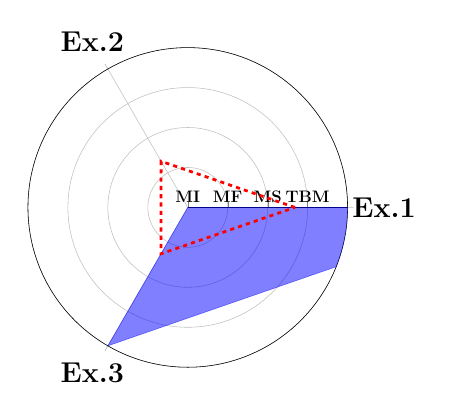
\begin{tikzpicture}[scale=0.5]
        \begin{polaraxis}[
            width=0.8\textwidth,
            xtick={0.0,120.0,240.0},
            xticklabels={\huge \bfseries Ex.1,\huge \bfseries Ex.2,\huge \bfseries Ex.3},
            ymin=0, ymax=100,
            ytick={0,25,50,75,100},
            yticklabels={\large \bfseries MI,\large \bfseries MF,\large \bfseries MS,\large \bfseries TBM, }
        ]
        \addplot+[mark=none,fill=blue,opacity=0.5] coordinates {
            (0.0,200.0)  (120.0,0.0)  (240.0,100.0)  
        } -- cycle;
        
        \addplot+[mark=none,fill=none,opacity=1,line width = 2pt,dashed,color=red] coordinates {
                    (0.0,67.0)  (120.0,33.333333333333336)  (240.0,33.5)  
                } -- cycle;
        
        \end{polaraxis}
    \end{tikzpicture}
\end{center}


    %%% fin - radar %%%

\end{multicols}

                \newpage
                
                \end{document}
            